
\subsection{Resumen de objetivos}

El objetivo del presente trabajo, es el análisis del amplificador de potencia de audio \textbf{Turner 730}, el circuito del mismo se muestra en la figura~\figref{fig:fig_complete_real_circuit}. El amplificador es un modelo que se comercializó hace varios años, pero que hasta hoy en día es buscado por aficionados al audio y es también construido en su versión original, o en varias variantes que se pueden encontrar en foros sobre audio.


\begin{figure}[H] %htb
\begin{center}
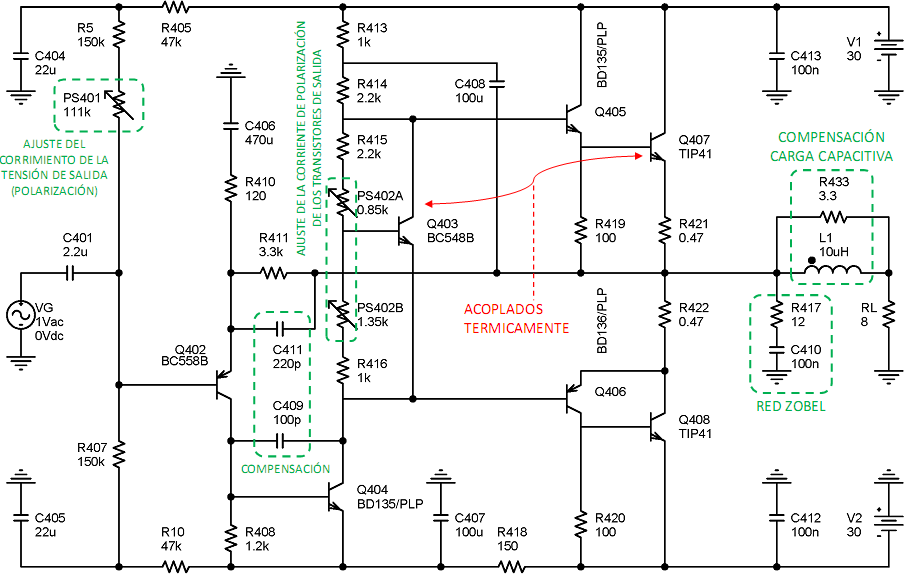
\includegraphics[width=0.9 \textwidth, angle=0]{./img/desarrollo/0_circuito_propuesto.png}
\caption{\label{fig:fig_complete_real_circuit}\footnotesize{Circuito del amplificador de potencia \textbf{Turner 730}.}}
\end{center}
\end{figure}




\subsection{Desarrollo}


El desarrollo se hace en base a los puntos del enunciado, pero básicamente es el mismo esquema que con cualquier circuito, primero se analiza en forma manual el punto de reposo de todos los transistores en la sección~\sectref{cacho}, para luego analizar el circuito en señal, encontrando la ganancia del camino directo, mediante el análisis de cada etapa, sección~\sectref{cacha}, luego se analiza la realimentación y se encuentra la ganancia de lazo, sección~\sectref{cacha}, ganancia global, sección~\sectref{cacha}, y así siguiendo con otras características del amplificador. Se hace también un análisis de potencia de los transistores de salida, para determinar si es necesario un disipador térmico, y de ser así cuál sería el indicado. Finalmente luego de los cálculos manuales, los mismos se verifican con un análisis por simulación con \textbf{SPICE} (\textbf{LTSPICE} en nuestro caso), a partir de la sección~\sectref{cacha}.






\clearpage